\documentclass{hw}

\usepackage{minted}

\begin{document}
\makeheader{}
\noindent\\

The logistic difference equation, governing population growth, is given by $x_{n+1}=rx_{n}(1-x_{n})$, in which
$r$ is the growth rate parameter. In the following exercises take the initial condition, $x_{1}$, to be
0.5.

\begin{enumerate}
\item Write a compute code (which utilizes either a for loop or a do loop) to analyze the behavior of the
logistic equation for $r=1.5$.

\vspace{0.5cm}

\begin{minipage}{0.5\textwidth}
\begin{minted}{python}
Population[r_, parg_: Automatic] :=
(
  x = Table[n, {n, 1, 200}];
  x[[1]] = 0.5;
  For[n = 2, n <= 200, n++,
   x[[n]] = r*x[[n - 1]]*(1 - x[[n - 1]])];
  ListPlot[x, PlotRange -> parg]
)
Population[1.5]
\end{minted}
\end{minipage}
\begin{minipage}{0.5\textwidth}
\centering
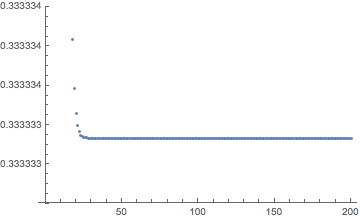
\includegraphics[scale=0.5]{p15}
\end{minipage}

\item Try several other values of the growth rate parameter in the range $1<r<3$. Do your results support
the conjecture that the limiting population always exists and is an increasing function or $r$?

\vspace{0.5cm}

{\centering
\begin{tabular}{c c c}
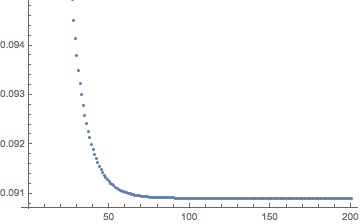
\includegraphics[scale=0.4]{p11}&
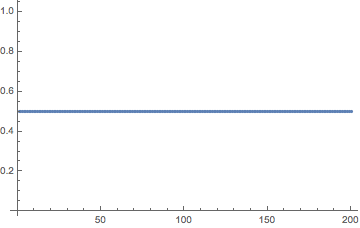
\includegraphics[scale=0.4]{p20}&
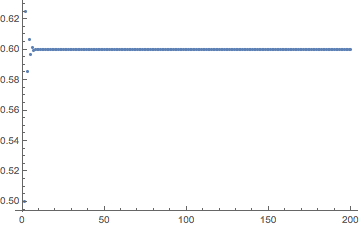
\includegraphics[scale=0.4]{p25}\\
$r=1.1$ & $r=2.0$ & $r=2.5$
\end{tabular}

\begin{tabular}{c c}
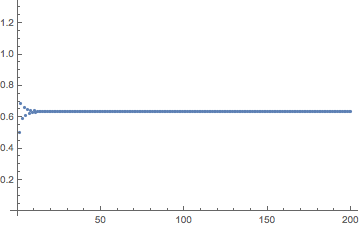
\includegraphics[scale=0.4]{p275}&
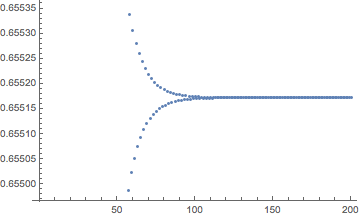
\includegraphics[scale=0.4]{p29}\\
$r=2.75$ & $r=2.9$
\end{tabular}
}

It's not always increasing, but the limiting population does always exist.

\newpage

\item Try values of the growth rate parameter in the range $2.9<r<3.1$ to determine as closely as possible
just where the single limiting population splits into a cycle of period 2.

\vspace{0.5cm}

{\centering
\begin{tabular}{c c c}
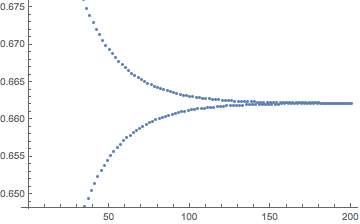
\includegraphics[scale=0.4]{p296}&
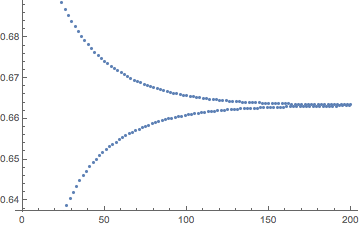
\includegraphics[scale=0.4]{p297}&
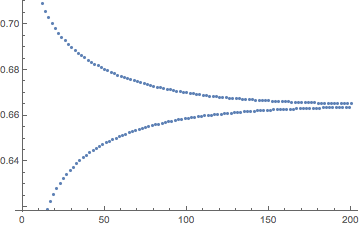
\includegraphics[scale=0.4]{p298}\\
$r=2.96$ & $r=2.97$ & $r=2.98$
\end{tabular}
}

The population appears to begin to split around $2.97<r<2.98$.

\item Verify that a cycle with period 16 is obtained with the growth rate parameter $r=3.565$.

\vspace{0.5cm}

\begin{minipage}{0.5\textwidth}
\begin{minted}{mathematica}
Population[3.565]
\end{minted}
\end{minipage}
\begin{minipage}{0.5\textwidth}
\centering
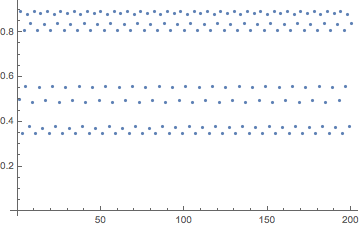
\includegraphics[scale=0.5]{div16}
\end{minipage}

\end{enumerate}
\end{document}
